\chapter{Modellazione degli oggetti concettuali con i Diagrammi delle Classi}
Sostanzialmente, questo modello rappresenta una vista \textbf{strutturale} del sistema che
vogliamo modellare (\textit{to-be}) o il sistema attuale che vogliamo analizzare 
(\textit{as-is}).

L'obiettivo è modellare i concetti, le strutture e i collegamenti tra i vari 
oggetti che rappresentano i requisiti del sistema.

La rappresentazione avviene tramite i \textbf{Diagrammi delle Classi} \texttt{UML}, declinandolo 
verso l'uso di una terminologia differente. Questo perché nella terminologia 
\textit{goal oriented}, quando parliamo di oggetti e classi, non ci riferiamo alla 
metodologia orientata agli oggetti, bensì modelliamo concetti del mondo reale.

L'oggetto \textit{treno}, o \textit{controllore} non si riferiscono al software, ma al mondo dei 
requisiti che stiamo modellando e, dato che non modelliamo il
software, \textbf{le classi non hanno operazioni}, ma solo \textbf{attributi} per modellare 
le proprietà degli oggetti del mondo che stiamo modellando.

\section{Oggetto concettuale}
\begin{tcolorbox}[colback=violet!5!white,colframe=violet!75!black, title=Oggetto concettuale]
    Un oggetto concettuale è un insieme di istanze che godono di queste proprietà:
    \begin{itemize}
        \item \textbf{sono identificabili in maniera distinta}
        \item \textbf{possono essere enumerati in ogni stato del sistema}
        \item \textbf{condividono caratteristiche comuni}
        \item \textbf{possono essere differire da uno stato all'altro}
    \end{itemize}
\end{tcolorbox}
Rappresentiamo lo stato di un oggetto di rappresenta con la lista di tuple $x_i \rightarrow v_i$,
dove:
\begin{itemize}
    \item $x_i$ è l'attributo dell'oggetto, associazione;
    \item $v_i$ è il valore dell'istanza.
\end{itemize}
\subsubsection{Esempio}
Per l'istanza \texttt{tr} dell'oggetto \texttt{Treno}:
\[
(tr.Speed \rightarrow 100, tr.Loc \rightarrow 9.25, tr.Dest \rightarrow MI,
On \rightarrow (tr, block13), At \rightarrow (tr, st1))
\]
La relazione tra gli oggetti e le istanze di oggetti è che 
un object instance è un'istanza di un oggetto, rappresentato come \texttt{instanceOf(o, Ob)}.
A differenza dell'object oriented, nel corso dell'evoluzione del sistema, un oggetto 
può diventare un'istanza di un altro oggetto. Un'istanza più essere membro di più 
oggetti (\textbf{tipizzazione multipla}).

\subsection{Classi e istanze correnti}
Nella rappresentazione diagrammatica, per ogni oggetto bisogna specificare obbligatoriamente 
la motivazione per cui un'istanza è istanza di un oggetto. 
\section{Entità}
\begin{tcolorbox}[colback=green!5!white,colframe=green!75!black, title=Entità]
    Un'entità è un oggetto \textbf{autonomo} e \textbf{passivo}, non controllano il funzionamento 
    e lo stato di altri oggetti. L'esistenza di tali oggetti è indipendente dall'esistenza di 
    altri oggetti. Tali oggetti vengono rappresentati attraverso le \textbf{classi} \texttt{UML}.
\end{tcolorbox}
\begin{figure}[H]
    \centering
    \begin{tikzpicture}
        \umlemptyclass{Treno}
    \end{tikzpicture}
    \caption{Esempio di entità}
\end{figure}
Necessitano della annotazione \textbf{Def}, che specifica la definizione dell'oggetto.
\section{Associazioni e molteplicità}
\begin{tcolorbox}[colback=blue!5!white,colframe=blue!75!black, title=Associazioni]
    Un'associazione è un oggetto concettuale che collega altri oggetti, ed ogni 
    oggetto ha un ruolo specifico. Tali oggetti si rappresentano mediante 
    le associazioni \texttt{UML}.
\end{tcolorbox}
\begin{figure}[H]
    \centering
    \begin{tikzpicture}
        \umlemptyclass{Train}
        \umlemptyclass[x=6]{Block}
        \umlHVassoc[name=assoc]{Train}{Block}
        \node at ($(Train.east)!0.2!(Block.west) + (0,0.2)$) {isOn};
        \node at ($(Block.west)!0.2!(Train.east) + (0,0.2)$) {hasTrain};
        %below assoc 
        \node at ($(Train.south)!0.5!(Block.north) + (0,-0.2)$) {\textbf{On}};
    \end{tikzpicture}
    \caption{Esempio di associazione}
\end{figure}
\begin{tcolorbox}[colback=blue!5!white,colframe=blue!75!black, title=Istanza di associazione]
    Un'istanza di associazione che collega due istanze di oggetti.
\end{tcolorbox}
In linea di principio possono riferirsi ad un numero arbitrario di oggetti, avendo un'arietà maggiore 
di due oggetti.
\subsection{Molteplicità}
La molteplicità è un vincolo che specifica il numero di oggetti che possono essere coinvolti
in un'associazione. La molteplicità può essere:
\begin{itemize}
    \item \textbf{0..1} - 0 o 1 oggetti
    \item \textbf{0..*} - 0 o più oggetti
    \item \textbf{1..*} - 1 o più oggetti
    \item \textbf{1..1} - 1 oggetto
\end{itemize}
\begin{figure}[H]
    \centering
    \begin{tikzpicture}
        \umlemptyclass{Patron}
        \umlemptyclass[x=10]{BookCopy}
        \umlHVassoc[mult1=0..1, mult2=0..*]{Patron}{BookCopy}
        \node at ($(Patron.south)!0.5!(BookCopy.north) + (0,-0.2)$) {\textbf{Loan}};
    \end{tikzpicture}
    \caption{Esempio di associazione con molteplicità}
\end{figure}
Possono anche essere riflessive, partendo da un oggetto e ritornando allo stesso oggetto.
\section{Eventi}
\begin{tcolorbox}[colback=cyan!5!white,colframe=cyan!75!black, title=Eventi]
    Un evento è un oggetto istantaneo, gli oggetti che sono istanze di eventi soddisfano 
    la proprietà \texttt{Occurs(Ev)}. Gli eventi sono rappresentati tramite gli 
    le classi \texttt{UML}.
\end{tcolorbox}
\begin{figure}[H]
    \centering
    \begin{tikzpicture}
        \umlemptyclass{BookRequest}
    \end{tikzpicture}
    \caption{Esempio di evento}
\end{figure}
\section{Agenti}
\begin{tcolorbox}[colback=gray!5!white,colframe=gray!75!black, title=Agenti]
    Un agente è un oggetto attivo e autonomo, che hanno funzionamento autonomo e
    possono \textbf{controllare} o \textbf{modificare} lo stato di altri oggetti, 
    causando transizioni di stato. Gli agenti sono rappresentati tramite
    le classi \texttt{UML}.
\end{tcolorbox}
\begin{figure}[H]
    \centering
    \begin{tikzpicture}
        \umlemptyclass{User}
    \end{tikzpicture}
    \caption{Esempio di agente}
\end{figure}
\section{Attributi}
\begin{tcolorbox}[colback=yellow!5!white,colframe=yellow!75!black, title=Attributi]
    Gli attributi sono proprietà degli oggetti che modelliamo, e sono rappresentati 
    mediante gli attributi delle classi \texttt{UML}.
\end{tcolorbox}

\begin{figure}[H]
    \centering
    \begin{tikzpicture}
        \umlclass{Train}{speed: float \\ dest: string \\ DoorState: \{open, \dots\}}{}
    \end{tikzpicture}
    \caption{Esempio di attributi}
\end{figure}
Anche le associazioni, in quanto oggetti, possono avere attributi.
\begin{figure}[H]
    \centering
    \begin{tikzpicture}
        \umlclass{Patron}{Phone [*] : String}{}
        \umlclass[x=10]{BookCopy}{CopyId: String}{}
        \umlHVassoc[name=assoc, mult1=0..1, mult2=0..*]{Patron}{BookCopy}
        \umlassocclass[geometry=|-|,x=5,y=2]{Loan}{assoc-1}{DateBorrow: Date \\ TimeLimit: NumberWeeks}{}
    \end{tikzpicture}
    \caption{Esempio di associazione con molteplicità}
\end{figure}

\section{Specializzazione}
\begin{tcolorbox}[colback=orange!5!white,colframe=orange!75!black, title=Specializzazione]
    La specializzazione è un'associazione tra una classe generale e una classe 
    specializzata, dove la classe specializzata eredita gli attributi della classe 
    generale. La specializzazione è rappresentata tramite l'ereditarietà delle classi 
    \texttt{UML}.
\end{tcolorbox}

\begin{figure}[H]
    \centering
    \begin{tikzpicture}
        \umlclass{Train}{speed: float \\ dest: string \\ DoorState: \{open, \dots\}}{}
        \umlclass[x=-3, y=-5]{Semi-Rapid}{}{}
        \umlclass[x=3, y=-5]{Rapid}{}{}
        \umlVHVinherit{Semi-Rapid}{Train}
        \umlVHVinherit{Rapid}{Train}
    \end{tikzpicture}
    \caption{Esempio di specializzazione}
\end{figure}
\subsection{Inibizione dell'ereditarietà}
In questo modo specializzare un oggetto, definendo un attributo in maniera 
più specifica rispetto all'attributo generale (\textit{si tratta di una ridefinizione}).
\begin{figure}[H]
    \centering
    \begin{tikzpicture}
        \umlclass{TrafficSignal}{color: \{red, yellow, green\} \\ Location: String}{}
        \umlclass[y=-3]{WaringSignal}{color: {yellow}}{}
        \umlVHVinherit{WaringSignal}{TrafficSignal}
    \end{tikzpicture}
    \caption{Esempio di specializzazione}
\end{figure}
\subsection{Ereditarietà multipla}
Un oggetto può essere specializzato in più oggetti, ereditando gli attributi
di più classi.
\begin{figure}[H]
    \centering
    \begin{tikzpicture}
        \umlclass{Strudent}{Email: String \\ StrudentId: String}{}
        \umlclass[x=6]{Patron}{Email: String \\ PatronId: String}{}
        \umlclass[y=-3, x=3]{StrudentPatron}{\dots}{}
        \umlinherit{StrudentPatron}{Strudent}
        \umlinherit{StrudentPatron}{Patron}
    \end{tikzpicture}
    \caption{Esempio di specializzazione}
\end{figure}
Possiamo avere dei conflitti, in questo caso, avendo il campo \texttt{Email} in entrambe
le classi, dobbiamo rinominare il campo in uno dei due oggetti.

\begin{tcolorbox}[colback=green!5!white,colframe=green!75!black, title=Benefici della specializzazione]
Una struttura basata su specializzazione permette di:
\begin{itemize}
    \item Avere un modello più semplice evitando la duplicazione di attributi.
    \item L'eliminazione di attributi è possibile su uniche entità evitando disallineamenti.
\end{itemize}
\end{tcolorbox}
\section{Aggregazione}
\begin{tcolorbox}[colback=teal!5!white,colframe=teal!75!black, title=Aggregazione]
    L'aggregazione è una composizione di diversi oggetti, dove ogni oggetto rappresenta una 
    parte. In questa relazione, l'oggetto aggregato può essere considerato un contenitore
    dei suoi componenti, ma i componenti possono esistere indipendentemente dall'aggregato.
\end{tcolorbox}
L'aggregazione è applicabile alle entità, agenti, eventi e associazioni.
Nelle relazioni di aggregazione, le molteplicità possono essere attaccate ai
collegamenti parte-aggregazione, suggerendo che una parte può essere condivisa
tra più aggregati o esistere in molteplicità variabili.
\begin{figure}[H]
    \centering
    \begin{tikzpicture}
        % Aggregazione
        \umlclass[type=abstract, x=0, y=0]{Library}{...}{}
        \umlclass[x=-3, y=-3]{Directory}{...}{}
        \umlclass[x=0, y=-3]{Shelve}{...}{}
        \umlclass[x=3, y=-3]{AntiTheft}{...}{}
        \umlVHVaggreg[]{Library}{Directory}
        \umlVHVaggreg[]{Library}{Shelve}
        \umlVHVaggreg[]{Library}{AntiTheft}
        % Composizione
        \umlclass[x=7]{Car}{...}{}
        \umlclass[x=7, y=-3]{Door}{...}{}
        \umlcompo[mult1=1, mult2=2..*]{Car}{Door}
      \end{tikzpicture}
\end{figure}

\subsection{Differenze tra Aggregazione e Composizione}
Mentre l'aggregazione permette che le parti esistano indipendentemente dall'aggregato,
la composizione è una forma più forte di aggregazione dove le parti non hanno
un'esistenza indipendente dall'aggregato. Se un aggregato viene distrutto, tutte
le sue parti vengono distrutte con esso. Questo legame è utile per rappresentare
relazioni vita o morte tra componenti, come tra un corpo e gli organi interni.

\subsection{Esempi di Aggregazione}
Un esempio comune di aggregazione potrebbe essere una libreria e i libri che
contiene. La libreria è l'aggregato, e i libri sono le parti. I libri possono
esistere al di fuori della libreria, suggerendo che la libreria è solo un
contenitore per i libri, non una necessità per l'esistenza dei libri.

Un altro esempio può essere un'azienda (\textit{aggregato}) e i suoi dipartimenti (\textit{parti}).
Mentre i dipartimenti sono funzionalmente parte dell'azienda, possono tecnicamente
operare in qualche misura indipendentemente dall'azienda stessa.
\section{Euristiche per la Modellazione degli Oggetti}

Nel processo di modellazione degli oggetti, è fondamentale seguire determinate 
euristiche per assicurare una progettazione chiara e funzionale. Di seguito sono 
elencate le principali linee guida da considerare:

\begin{itemize}
  \item \textbf{Revisione delle Specifiche}: È cruciale rivedere tutte le specifiche 
  degli obiettivi e delle proprietà del dominio contenute nel modello degli obiettivi 
  per garantire che tutte le necessità siano adeguatamente rappresentate e comprese.
  
  \item \textbf{Assegnazione degli Obiettivi}: Per l'implementazione degli obiettivi 
  nel software da realizzare, è essenziale introdurre rappresentazioni condivise degli 
  oggetti dell'ambiente riferiti dagli obiettivi.
  
  \item \textbf{Definizione degli Attributi}: Un elemento è da considerare un attributo 
  se è una funzione che restituisce un valore unico, le sue istanze non necessitano 
  distinzione, non si prevede di aggiungervi attributi o associazioni, e non si 
  intende specializzarne l'intervallo di valori.
  
  \item \textbf{Oggetti Concettuali negli Obiettivi}:
  \begin{itemize}
    \item Gli oggetti concettuali definiti da uno stato unico 
    (esempio: \textit{StartTrain}) implicano eventi.
    \item Gli oggetti che attivano e controllano comportamenti di altre 
    istanze (esempio: \textit{DoorsActuator}) agiscono come agenti.
  \end{itemize}
  
  \item \textbf{Attributi nelle Associazioni}: Un attributo deve essere 
  collegato a un'associazione se caratterizza tutti gli oggetti partecipanti, 
  sia esplicitamente che implicitamente.
  
  \item \textbf{Link Strutturali e Associativi}: Considerare la creazione di 
  un'associazione se esiste un link strutturale tra oggetti compositi e 
  componenti che soddisfa specifiche condizioni operative o strutturali.
  
  \item \textbf{Specializzazioni e Generalizzazioni}: È importante identificare 
  specializzazioni e generalizzazioni attraverso l'analisi di attributi comuni, 
  associazioni e invarianti di dominio, contribuendo alla creazione di un modello 
  più organizzato e scalabile.
  
  \item \textbf{Uso di Associazioni invece di Puntatori}: Evitare l'utilizzo 
  di ``puntatori" agli altri oggetti come attributi e preferire l'uso di 
  associazioni binarie.
  
  \item \textbf{Nomi e Definizioni Chiare}: Utilizzare nomi suggeriti e 
  chiari per oggetti e attributi, evitando ambiguità e assicurando una 
  definizione precisa e dettagliata.
\end{itemize}